\documentclass{ctexart}

\usepackage{amsmath}

\usepackage{amsthm}

\usepackage{amssymb}

\usepackage{bm}

\usepackage{graphicx}

\usepackage{listings}
\lstset{
basicstyle=\scriptsize
}

\usepackage{caption}

\begin{titlepage}

\title{微分方程数值解 \\ 第十一周作业}

\author{于慧倩 \\ 14300180118}

\date{2017年5月}

\end{titlepage}

\begin{document}

\maketitle

\newpage

\begin{enumerate}

\item P164.1

 在区域\(\Omega = [0,1]^2\)用五点差分格式求解如下问题:
 
\[
-\Delta u +u =fs
\]

且\(u|_{\partial \Omega} = 1\) ,设\(\bm{A}\)为对应\(-\Delta\)算子的离散矩阵,说明:
\begin{enumerate}
\item 观察\(\bm{A}+\bm{I}\)的性质:


进行五点差分,把\(x,y\)方向\(N\)等分,步长为\(h=1/N\),在内部节点上
\[
\Delta_h u_{i,j} = \frac{1}{h^2}(u_{i+1,j}+u{i-1,j}+u_{i,j+1}+u_{i,j-1}-4u_{i,j})
\]

若边界条件为\(u|_{\partial \Omega} =0\),则有

\begin{equation*}
\bm{S}={
\left ( \begin{array}{ccccc}
4 & -1 &0  & &  \\
-1& 4 & -1 & \ddots& \\
  &-1& 4&\ddots & \\
  & &\ddots &\ddots &-1\\
  &  & &-1 &4
\end{array} 
\right )_{N-1,N-1}}
\end{equation*}
 
 \begin{equation*}
\bm{T}={
\left ( \begin{array}{ccccc}
 -1&  & & &  \\
 & -1 & & & \\
  & & -1&& \\
  & & &\ddots &\\
  &  & & &-1
\end{array} 
\right )_{N-1,N-1}}
\end{equation*}

 \begin{equation*}
\bm{A}=\frac{1}{h^2}{
\left ( \begin{array}{ccccc}
S&T  &S & &  \\
T & S & T& & \\
  & T& S&\ddots & \\
  & &\ddots  &\ddots &T\\
  &  & &T &S
\end{array} 
\right )}
\end{equation*}


\(A+I\)的性质:对称,正定;只在五条对角线上的元素不为零,对应着每个节点只有五点进行计算;稀疏,块三对角阵;不可约;严格对角占优阵;

\item 格式是否两阶收敛

构造\(u=x(1-x)y(1-y)+1\)对应\(f=2y(1-y)+2x(1-x)+x(1-x)y(1-y)+1\),利用五点差分格式进行估计,得到误差如图:

\centerline{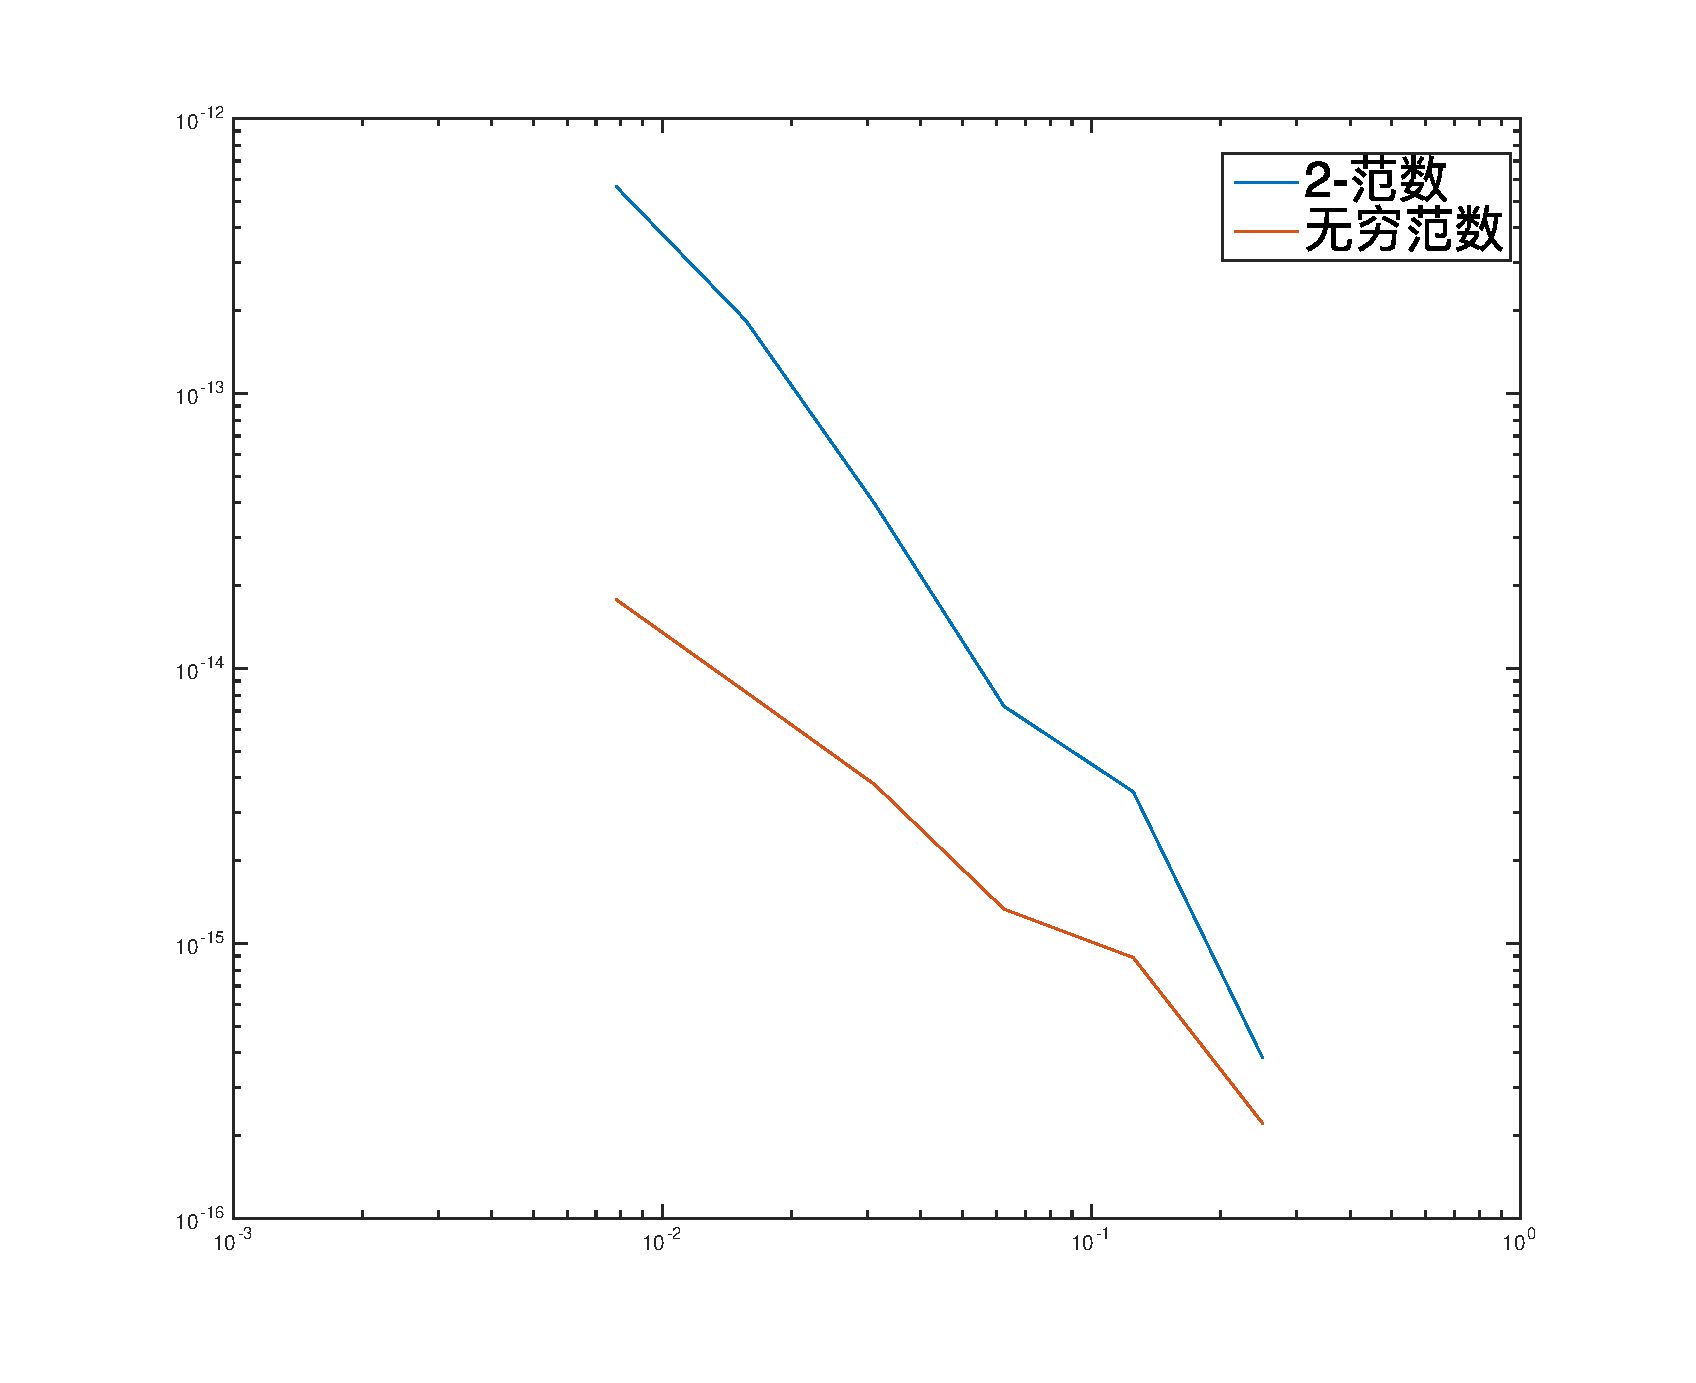
\includegraphics[width=5.5in]{H11_1.eps}}

可以看出符合二阶收敛。

\item 求矩阵\(A\)的特征值、特征向量

特征值:\(\lambda_{j,k}=\frac{4}{h^2}\mbox{sin}^2(\frac{j \pi}{2n})+\frac{4}{h^2}\mbox{sin}^2(\frac{k \pi}{2n})\)。其中\(j,k=1,\dots,N-1\)

对应的特征向量\(u_{m,l}^{(j,k)}=\frac{2}{n}\mbox{sin}(\frac{mj \pi}{n})\mbox{sin}(\frac{lk \pi}{n})\)。其中\(1 \leq m,l\leq N-1\)
\end{enumerate}













\end{enumerate}
\end{document}